\documentclass[journal, a4paper]{IEEEtran}

\usepackage{graphicx}
\usepackage{url} 
\usepackage{subcaption}
\usepackage{multicol}
\usepackage{float}


\begin{document}

\title{Open Data Innovation Group Report}
\author{Thomas Aley, ta2g12.\\
Shakib-Bin Hamid, sh3g12.\\
Stefan Collier, sc22g13.\\
Lendina Hykaj, lh6g13.\\
Deepak Thankachan, dt9g13.}
\maketitle

\begin{abstract}
Having no fast and stable means of accessing all of the University of Southampton (UoS) open datasets, members of UoS under-utilize these services. Soton Bot is a chatbot that combines these datasets and serves them through a single location. The bot can give concise and relevant answers to questions regarding the university; whether it is about locations of buildings, bus times or the nearest petrol station. Facebook Messenger was chosen to host the bot due to the wide popularity of the platform. \texttt{API.ai} was used to capture intent from natural language text. Soton Bot is a faster and more friendly alternative to access the existing sources of information about campus life. Also, as a platform, it can benefit organisations in delivering their open data.
\end{abstract}

\section{Introduction}
Soton Bot is a chatbot on Facebook Messenger that answers natural language queries about things around University of Southampton, such as room booking, bus times, places to eat and find essentials, etc. using open data.\\

The university has opened up a large amount of data which is served through various different websites and services. Unfortunately, most people on campus are not aware of this information and the provisioning of these websites takes considerable effort. Furthermore, the users do not receive concise answers. For example: to find a free room, they would typically fill in a page long web form, where one would simply want an answer to the question - \textit{``Where can I get a room booking next week Monday?''}.\\

Chatbots are not a new concept. But unlike historical chatbots, Soton Bot is able to process natural language and extract information using modern AI technology. At the same time, Facebook Messenger is a reliable and popular messaging platform used by most people on campus. So, users will not have to use yet another unknown service from the university. Finally, it demonstrates a novel and exciting way to deliver an organisation’s open data, thus providing an opportunity to release Soton Bot as a platform.
    
\section{Background}

Advancements in technology have had an impact on how businesses and institutions interact with their clients. The implementation of Artificial Intelligence techniques on different platforms has made it easier for people to communicate with their chosen business. A chatbot is a software application that simulates human interaction by running automated scripts over the internet. Chatbots could live in most major messaging products such as Facebook Messenger, Slack, SMS, Skype or  WhatsApp.\\ 

Chatbots provide ease of use due to their incorporation in messaging platforms that the users would have already downloaded. Instead of the user downloading a new application, they could just add a new bot contact. In addition, they are extremely easy to use due to the usage of natural language. They provide the user with immediate personalized answers at all times. The bot retrieves information from secure data sources which provides the user with correct information. In addition, bots reduce costs significantly. Instead of having many different websites that provide information, bringing it all together on one application is very cost-efficient.\\ 

One of the main reasons why these applications are a huge opportunity at the moment is because for the first time people are using messaging apps more than they are using social networking sites \cite{msgAppsData}. WhatsApp and Facebook Messenger have roughly the same amount of monthly active users \cite{statsPortal}. Facebook Messenger has a more interactive API which makes it easier for developers. Also, Facebook Messenger bot API has been around for longer and has been evolving rapidly \cite{botware}. Since Facebook Messenger is used on Facebook, it makes it easier for bot developers to advertise their products.\\ 

Facebook Messenger already has a significant amount of chatbots available to the public. They are mostly concentrated towards retail and fashion. However, there are many bots that provide the users with services such as the Skyscanner Bot which allows the user to ask for different holiday or flight preferences \cite{skyscanner}. Having these bots on Facebook Messenger is very useful as it is an application that users would most likely have on their phones. 

\section{Data} 
\label{data}

\subsection{Sources}

We only use open data in Soton Bot. The primary source is the UoS open data. The datasets we have used include - Buildings \& Places, City Council Car Parks, Bus Information, Room Bookings, Food \& Drinks Outlets, Common Learning Spaces Info, Local Amenities, Photographs of UoS Things and a number more.\\

We also used two external sources - Open Street Map and Transport API. Open Street Map is a well known geographical open data service. We used it to provide locations of places on a map. Transport API is the most widely known UK transport open data provider, used by TFL, Heathrow, National Rail and more. While it is a paid service, 30 thousand hits are free every month. 

\subsection{Queries}

University of Southampton provides a \texttt{SPARQL} Endpoint \cite{sparql_endpoint} which can be used to query the triple store hosting all of the university's Open Data catalogues \cite{data_catalog}. We created \texttt{SPARQL} queries which could be used at this endpoint for data retrieval.\\

We utilised 2 APIs from Open Street Map: one for retrieving a static image and the other for a URL to an interactive map. By using the longitude and latitude, Open Street Map's RESTful service provides detailed map images. We signed up with Transport API and obtained a key to use their RESTful API for obtaining nearest bus stop location. 

\section{Design Decisions}
\subsection{Chatbot}
% ----------------------------------------------------------------------------------
% ----------------------------------------------------------------------------------
% -------------------------[ Why a chatbot ]----------------------------------------
% ----------------------------------------------------------------------------------
% ----------------------------------------------------------------------------------
We needed to find a suitable method for users to interact with the chatbot. The delivery of information must be fast, intuitive and simple. The following were considered: SMS, Applications, Websites and Messaging Platforms.\\

SMS provides the largest reach as it will be accessible everywhere within the context (Southampton). However, the interaction costs will expectedly accumulate to a significant amount.\\

Hosting the bot on a website and providing a text chat interface is much less costly. However, we would create yet another website for university data - the same problem we are trying to avoid.\\

Then we arrived at a mobile application which reduces website hosting fees. App development allows for a very personal look and feel to the service. But it requires the user to download a new app on their phone, a reiteration of the existing problem.\\

Finally, we chose a messaging platform, Facebook Messenger, as our delivery system. We can safely assume that the users already have it installed on their phones. The look and feel is also well established. This solution reduces a lot of costs since we do not have to provision delivery of the messages which is known to be robust.

\subsection{Natural Language}
We realised that the bot needed to understand human questions, as it would greatly improve the User Experience (UX). It would also make the bot more versatile compared to bots that only support simple command-like speech, e.g. \textit{``locate building 32''}. So, we had to choose whether to \textit{create} or \textit{use} a Natural Language Processor (NLP). \\

Creating a NLP would require a large amount of time and most likely involve creating a complex Machine Learning (ML) model and great amounts of training data. This effort would require the entire team much longer than the allocated time. It will also unlikely be as stable as some of the existing industry favourite services. \\

Hence using a hosted service is the feasible solution. A number of online services were considered and only \texttt{init.ai} and \texttt{API.ai} were shortlisted. These two services significantly reduce the training data required and also extrapolate from the small training statements to find synonyms and similar sentences. After creating simple prototypes, ultimately \texttt{API.ai} was chosen. It opens up most of its engine's internal workings to the developers, which gives it versatility and best of all, its functionality is available over a web API.

\subsection{User Experience}
UX was considered on every step of the design and implementation process. Garrett's UX \cite{garrett} theory was considered as a basis before any important UI decisions were taken. The main objective was to provide an application that most members of the university would keep coming back to.\\

The scope of this project could have been very vast, however we chose to focus on the most crucial aspects of student life as a starting point. The questions that can be asked to the bot relate to the life on campus. Since, the user would be able to chat to the bot in natural language, it could be assumed that the user would know how to interact with the system already. It can make the bot desirable to the public due to the simplicity of usage.\\

The answers that are given to the user are usually customised with pictures which make the interaction visually stimulating. For example if the user were to ask the bot ``What can you do?'', the bot would answer with customised images of what it is able to perform (As shown in \textbf{Fig \ref{fig:wf:skills}}).\\

\begin{figure}
	\centering
    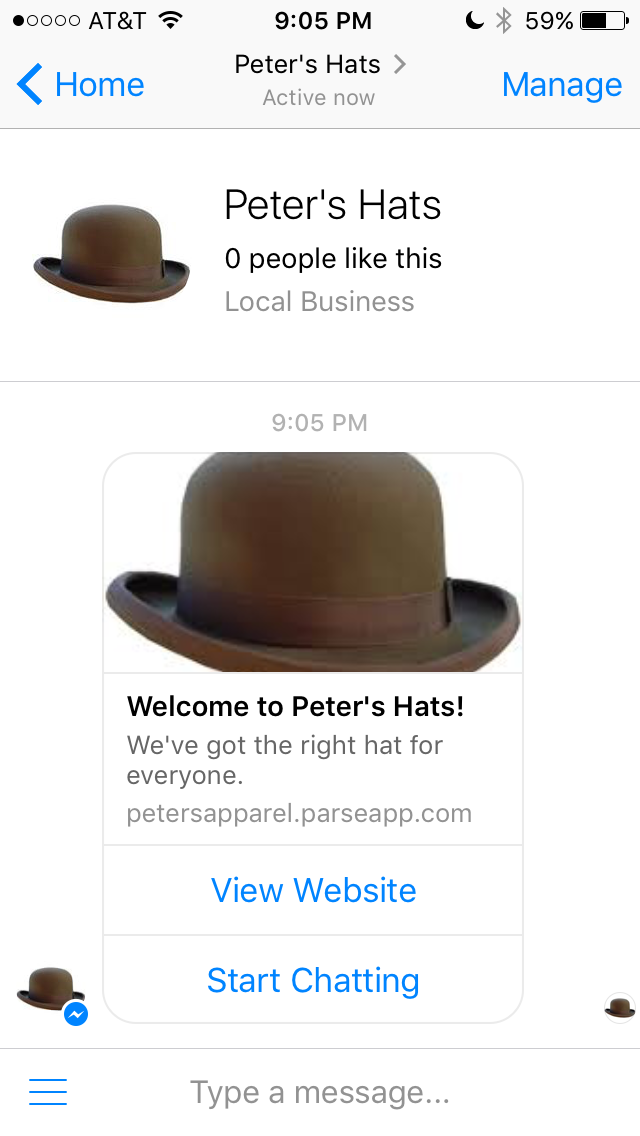
\includegraphics[width=0.2\textwidth]{images/example}
	\caption{Facebook Messenger Template Example}
    \label{fig:3:messenger_template}
\end{figure}

As the developer example (\textbf{Fig \ref{fig:3:messenger_template}}) had shown this was possible, a number of wireframes were created using the background research on existing chatbots to help create tasteful interactions. You can see our wireframes compared to the end result in \textbf{Figs \ref{fig:wf:skills}, \ref{fig:wf:services} and \ref{fig:wf:building}}.

\begin{figure}
	\centering
    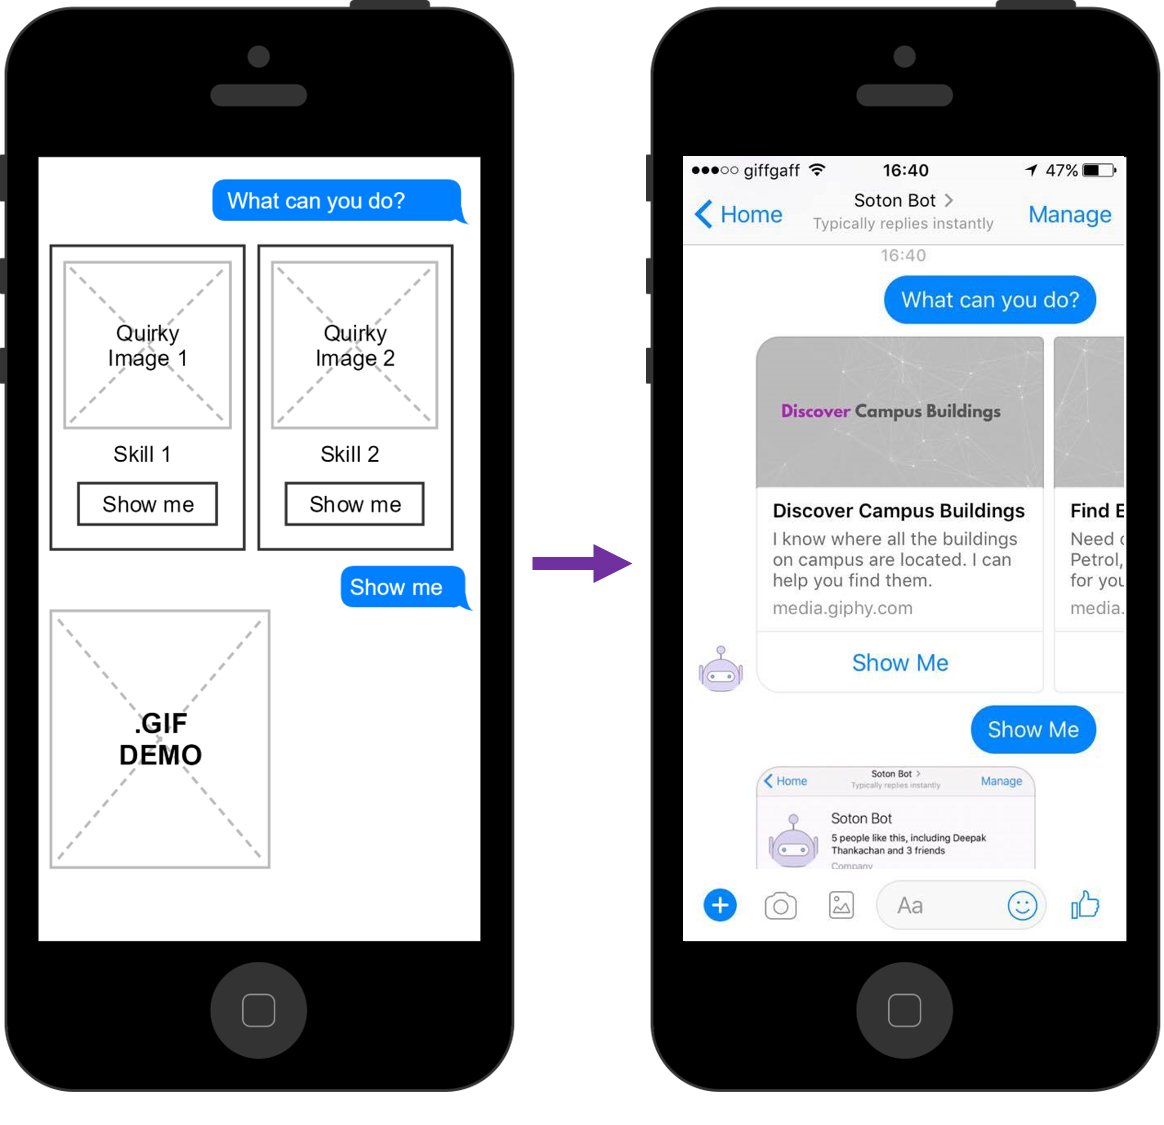
\includegraphics[width=0.45\textwidth]{images/wf-skills}
    \caption{{\small Find Bot Skills}}    
    \label{fig:wf:skills}
\end{figure}
\begin{figure}
	\centering
    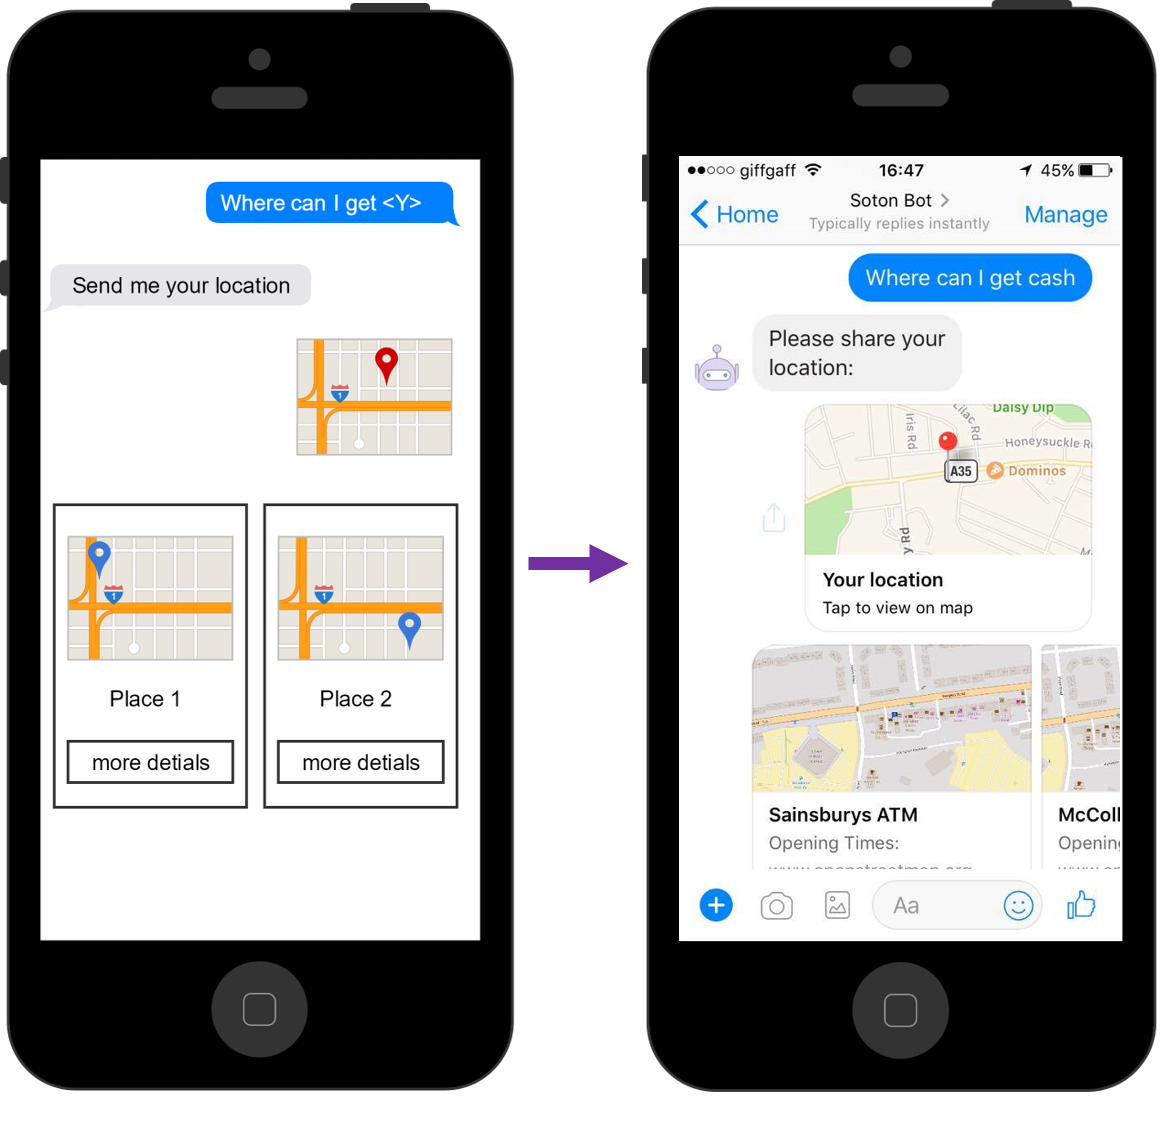
\includegraphics[width=0.45\textwidth]{images/wf-services}
	\caption{{\small Locate Services}}   
    \label{fig:wf:services}

\end{figure}
\begin{figure}
	\centering
    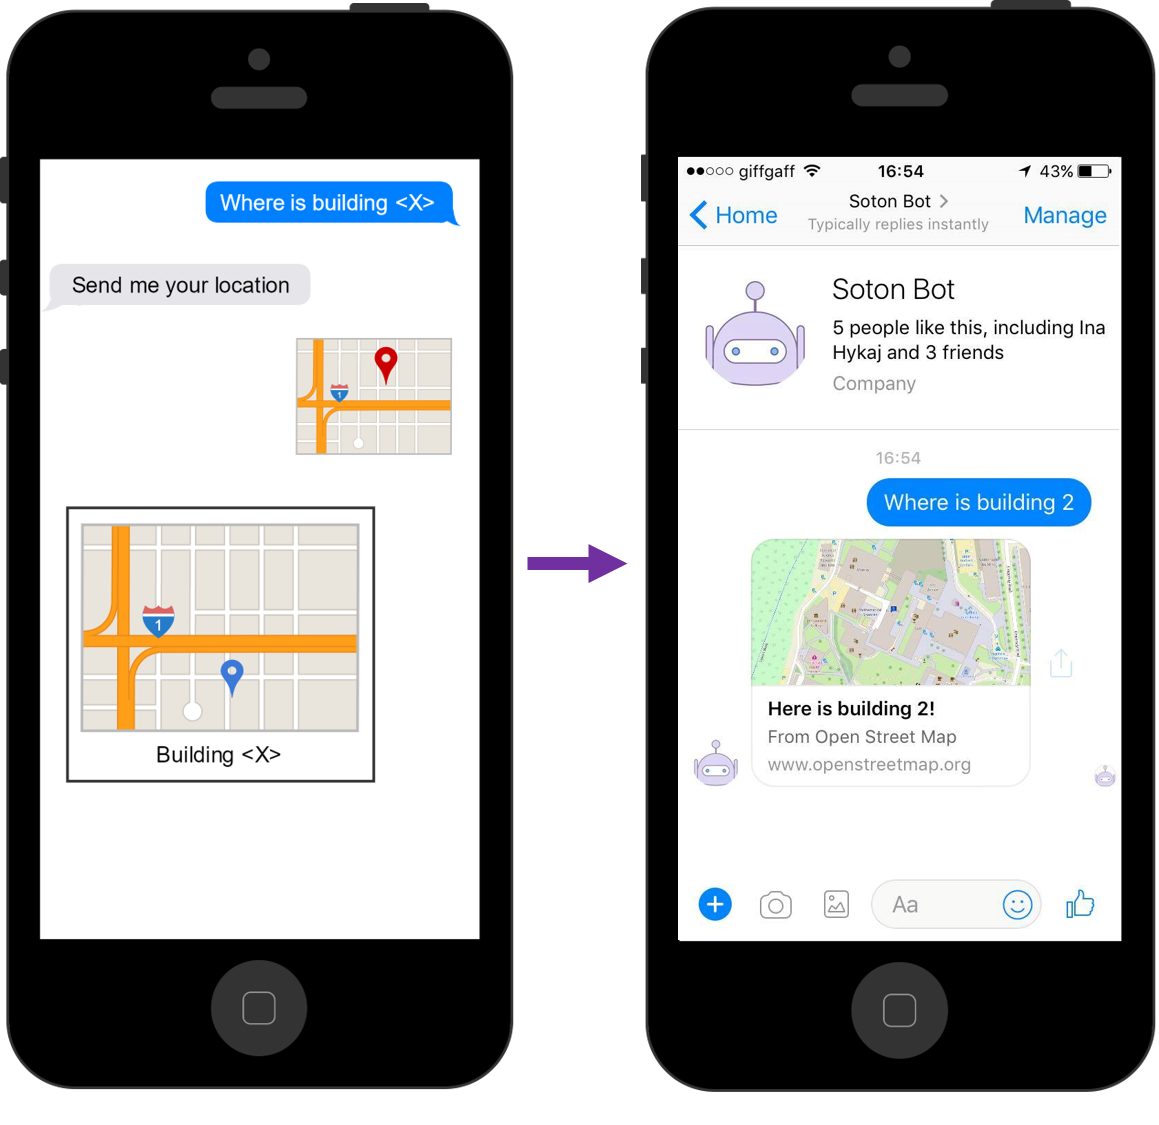
\includegraphics[width=0.45\textwidth]{images/wf-building}
	\caption{{\small Find a Campus Building}} 
	\label{fig:wf:building}
\end{figure}

The average user of the application would be a member of the University of Southampton. We made an assumption regarding what kind of information they would need from the application. Students and staff would need to know where buildings and rooms are as well as how they would be able to book a room. Also, public transport data needed to be incorporated. Food and drinks are another crucial aspect of student life in general. We believed that these were very important due to the different scenarios that this application was made for (see Appendix A).

\section{Implementation}

\begin{figure}
	\centering
    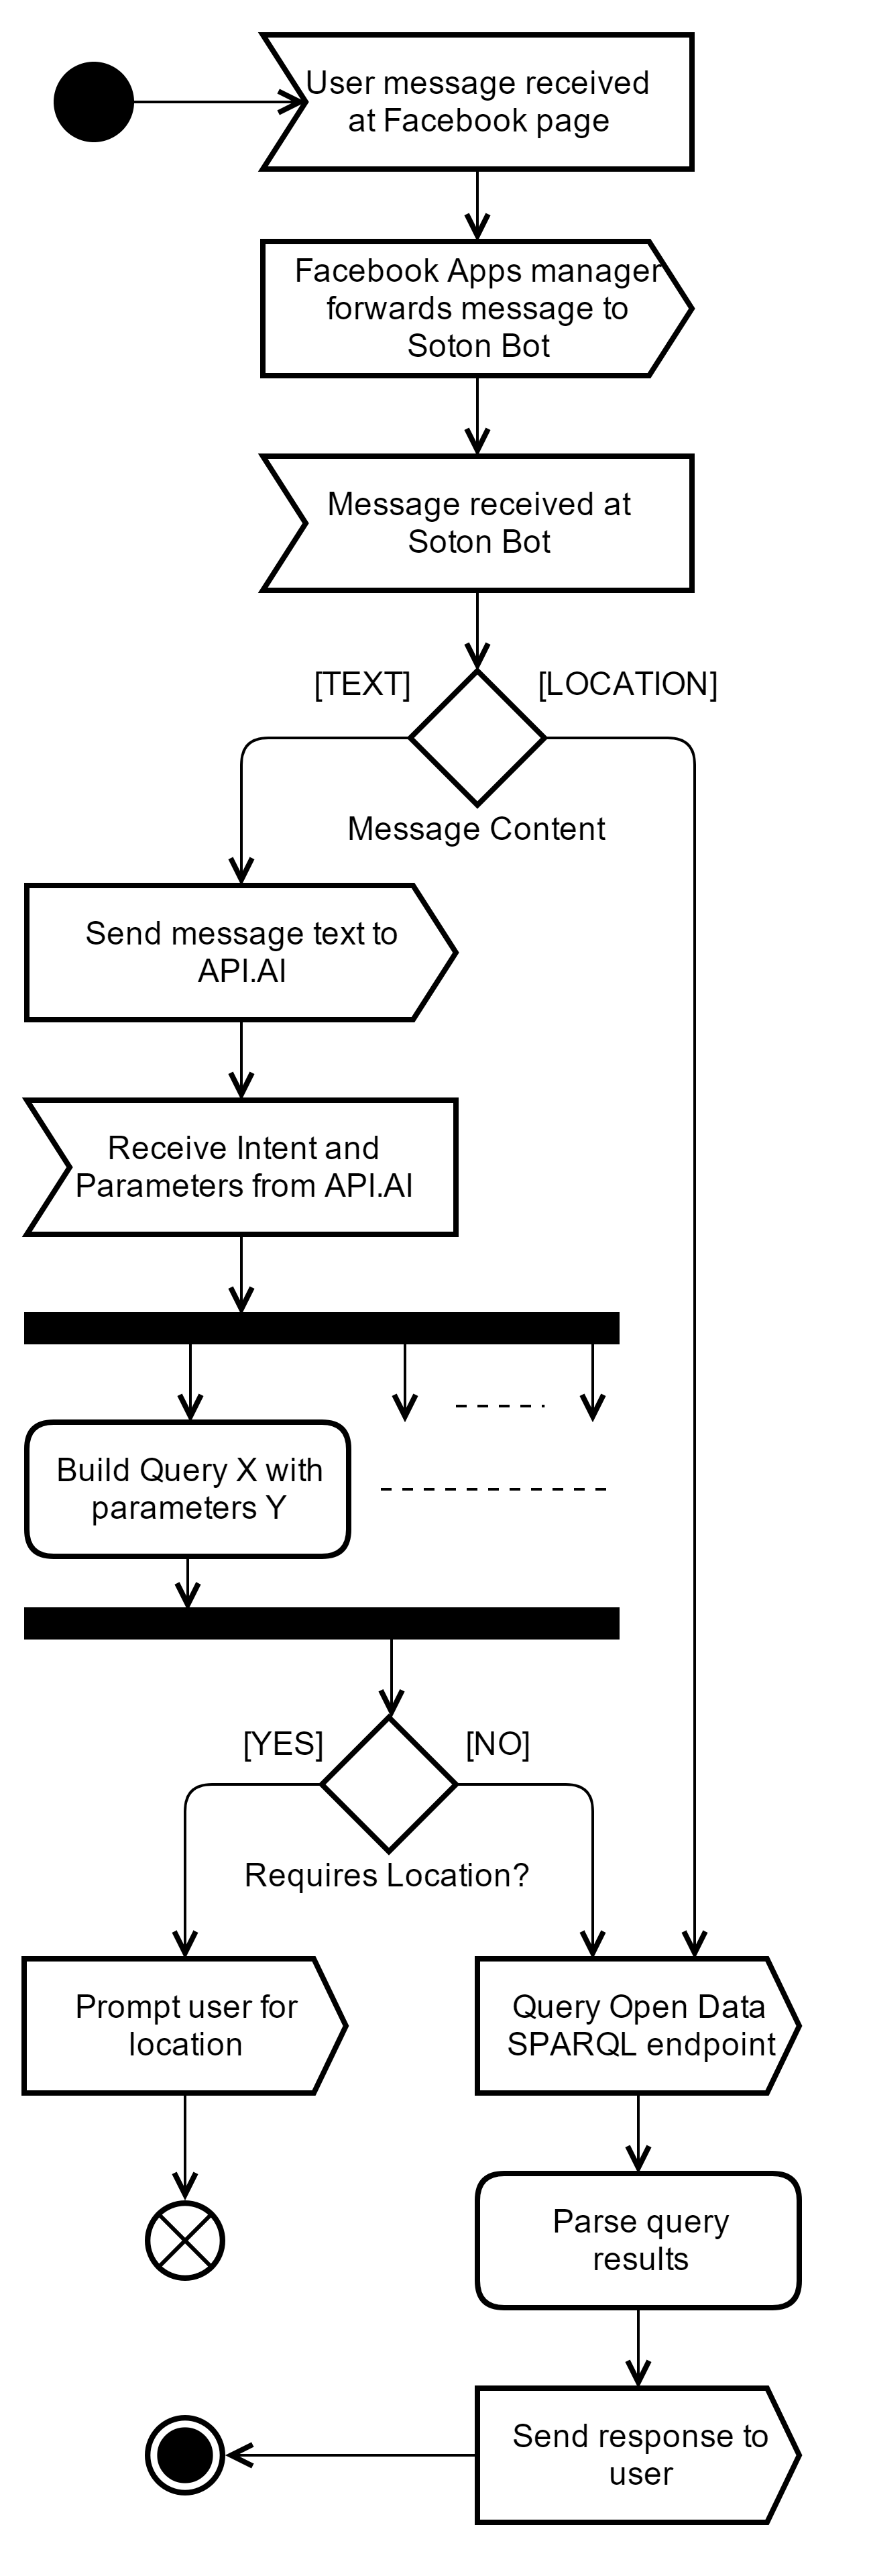
\includegraphics[width=0.4\textwidth]{images/activitydiagram.png}
   	\centering
	\caption{Activity diagram depicting the control flow of Soton Bot. Note that the 'end flow' symbol indicates the flow should begin again from the start node with location based message content.}
    \label{fig:activity_diagram}
\end{figure}

Soton Bot's implementation is not trivial, \textbf{Fig. \ref{fig:activity_diagram}} exists to depict the control flow of the application over the following sections. 

\subsection{App Initialisation}
Soton Bot's architecture involves many components. Before a message even reaches our \texttt{NodeJS} implementation of Soton Bot, it arrives at Soton Bot's Facebook business page. This page has a Messenger App associated with it and a webhook defined which points to our code base hosted on \texttt{Heroku}. This much is solely configuration, the complexity begins as the message arrives at our code.\\ 

\subsection{Determining Intent}
The first step in processing a message is to determine if the message is text based, some kind of attachment message (such as location information) or simply a message confirming the receipt of a response Soton Bot sent. With text based messages, we used \texttt{API.ai} to determine the intent behind the user's message and what variables we might need to extract. For example \textit{``Where's building 32?''} and \textit{``Where can I find the building 32''} would both result in the `\texttt{find-campus-building}' intent with the parameter \texttt{building\_number: 32}.\\

API.ai lets us review all training conversations with the bot. We can reclassify any messages that were incorrect to ensure that the parameters and intents would be correct in subsequent similar messages. Thus we helped it better understand spelling, auto-correct mistakes and  slang. Now the bot knows \textit{``Gimme some munch''} should result in finding the nearest places to eat.\\ 

\subsection{Triggering Actions}
The resulting intents and parameters provided by \texttt{API.ai} trigger appropriate actions in Soton Bot. These actions range from finding a building or free room to listing places which sell alcohol and how far they are from the user's current location. When a user's question requires a location to answer appropriately, \texttt{API.ai} signals \texttt{action\_incomplete} to Soton Bot which can then ask the user to provide a location to fulfill their request.\\ 

\subsection{Querying for Data}
The data described in \textbf{Section} \ref{data} is used to answer user's questions. In order to obtain data from Southampton university's \texttt{SPARQL} endpoint, we needed a way to dynamically build syntactically correct \texttt{SPARQL} queries using the provided parameters. The solution involved writing skeleton queries that we could store in \texttt{JSON} using a schema of our own design. JavaScript functions could then swap in parameters on demand and parse the \texttt{JSON} query using our custom JSON-SPARQL query converter, then HTML encode it and send it to the endpoint.\\

\subsection{Parsing Query Results}
Data returned from the endpoint is parsed to extract the most relevant subset of information. Our queries have been designed for efficiency so  little to no irrelevant data is returned, however there are limitations on what \texttt{SPARQL} is capable of. As such we further prune the results based on a user's location to only return results located within 250m of the user.\\ 

\subsection{Responding to Users}
The final task for Soton Bot's code is to transform the parsed data into a presentable format. We utilised Facebook Messenger Templates when we wished to send images with accompanying text, buttons or links for a richer interface. Finally Facebook's Graph API handles the sending of our responses.\\ 

\section{Testing}

\texttt{Mocha}\cite{mocha} was chosen as the test runner for our NodeJS application, complimented by the \texttt{Chai}\cite{chai} assertion library. As many of Soton Bot's capabilities require communication with external services, \texttt{Sinon}\cite{sinon} was used to stub these methods, override return values and spy on method calls.\\

Unit tests were written against stored query skeletons to ensure parameters were correctly added and that the resulting queries were syntactically correct. The majority of the remaining 30+ tests were integration tests ranging from tests of the responses from \texttt{API.ai}\cite{api_ai} to tests of our custom JSON query converter. We test \texttt{API.ai} by dynamically generating test cases based on example natural language questions and assert against expected intentions and parameters.\\

Aside from comprehensive automated testing as discussed above, we also used the bot regularly to test its functions and help us better train the AI.

\section{Future Work}

Lecture and lab schedules should be open data. We appreciate that a personnel's association with modules is personal data and therefore cannot be open. But we find no reason to not open up the data about the time and place for lectures/labs. For example: COMP6212 has a lecture in 46/2001 at 12pm on 13/05/2017. Our reasoning is that anyone can walk up to the campus and look on the room door for the timetable. So, why not make it open data to support queries such as \textit{``Where/When is the COMP6212 Lecture?"}, a common query amongst students.\\

We would like to support multiple languages. This will require significant AI training, but no extra work on the queries.\\

Gamifying the system to gather open data through crowdsourcing is possible. For example: the university does not have good data on building access, toilets, showers etc. We suggest starting a secondary editable triplestore, where the users can add data by talking to the bot. For example: \textit{``There's a shower in building 53. It's room number is 53/3033"} will add few triples to describe this information. If a dataset gets enough traction, then the open data team can decide on making the data authoritative. Every x number of correct insertions can reward the user.\\

We want to abstract the code regarding sending and receiving messages into a module. Our app will essentially become a platform, of which Soton Bot will be an implementation using Facebook Messenger. This way we would be able to support Slack, Skype, Hipchat, etc. chatbots as well, and give the functionality to hot swap communication modules for any business needs.\\

We also want to abstract the data retrieval code into a module. Our university data will be a source of this module. The queries will have a property of execution location which will point to one or more of such sources. This way we would be able to cleanly support multiple  different data sources at the same time. For example: query university open data and wikidata without changing the underlying architecture.\\

Submitting the bot for review on Facebook API (and passing the review) would allow it to be used publicly.

\section{Business Viablity}

In its current iteration, Soton Bot can instantly save the University hefty maintenance fees upon its deployment, since a large portion of its functionalities are performed by reliable external services. The university's open data is currently served on a plethora of websites, most of which the students are unfamiliar with, preventing the services from being fully utilised. Soton Bot fuses different datasets as an intuitive one stop shop, enabling the university to reduce resources to the current dedicated websites. Hence, saving on hosting fees.\\     

If the future work is implemented, it opens up the possibility of marketing the outcome as a framework which can be distributed to other  organisations. Soton Bot will then essentially be an implementaton of this framework for this university. The ability to hot swap datasets and messaging services will make the framework very powerful and allow hassle free adoption for 3rd parties, which is sure to stir up their interest.  

\section{Conclusion}

Soton Bot is a demonstration of some of today's most promising technologies. Intention and parameter extraction from natural language is now more accessible to us than ever before. So, we can create intuitive, informative and overall useful chatbots. There are a number of reliable and widely used communication APIs that have opened up platforms to build custom chat apps. Their proven infrastructure makes provisioning to provide reliable communication much less of a burden. Using both of the above makes developing and maintaining Soton Bot a pleasure. Finally, Soton Bot as a platform can help companies take advantage of their open data and encourage them to open up more of their data. We also hope that the exciting technologies used in Soton Bot will encourage future students and developers to build interesting and fun open data based applications.

\begin{thebibliography}{5}

	\bibitem{sparql_endpoint}
    iSolutions. 
    \emph{\texttt{SPARQL} Endpoint $\vert$ Open Data Service $\vert$ University of Southampton}. 
    [Online] Available at: 
    \url{http://sparql.data.southampton.ac.uk}.
    [Accessed 12 May 2017].\\
    
    \bibitem{data_catalog}
    iSolutions.
    \emph{Data Catalogue $\vert$ Open Data Service $\vert$ University of Southampton}.
    [Online] Available at:
    \url{http://data.southampton.ac.uk/datasets.html}.
    [Accessed 12 May 2017].\\
    
    \bibitem{mocha}
    Holowaychuk, T. J.
    \emph{Mocha - the fun, simple, flexible JavaScript test framework}.
    [Online] Available at:
    \url{https://mochajs.org/}.
    [Accessed 12 May 2017].\\
    
    \bibitem{chai}
    Luer, J.
    \emph{Chai Assertion Library}.
    [Online] Available at:
    \url{http://chaijs.com/}.
    [Accessed 12 May 2017].\\
    
    \bibitem{sinon}
    Sinonjs.org.
    \emph{Sinon.JS - Standalone test spies, stubs and mocks for JavaScript. Works with any unit testing framework}.
    [Online] Available at:
    \url{http://sinonjs.org}.
    [Accessed 12 May 2017].\\
    
    \bibitem{api_ai}
    api.ai.
    \emph{Conversational User Experience Platform}.
    [Online] Available at:
    \url{https://api.ai/}.
    [Accessed 12 May 2017].\\
    
    \bibitem{garrett}
    Garrett, J. J.
    \emph{The Elements of User Experience}.
    [Online] Available at:
    \url{http://www.jjg.net/elements/pdf/elements_ch02.pdf}.
    [Accessed 12 May 2017].\\
    
    \bibitem{msgAppsData}
    Business Insider.
    \emph{Messaging apps are now bigger than social networks}.
    [Online] Available at:
    \url{http://uk.businessinsider.com/the-messaging-app-report-2015-11}.
    [Accessed 12 May 2017].\\
        
    \bibitem{statsPortal}
    The Statistics Portal.
    \emph{Most popular mobile messaging apps worldwide as of January 2017, based on number of monthly active users (in millions)}.
    [Online] Available at:
    \url{https://www.statista.com/statistics/258749/most-popular-global-mobile-messenger-apps/}.
    [Accessed 12 May 2017].\\
    
    \bibitem{botware}
    Scocco, Daniel.
    \emph{Messenger and WhatsApp Chatbot Development}.
    [Online] Available at:
    \url{https://www.botware.com.br/messenger-and-whatsapp-chatbot-development/}.
    [Accessed 12 May 2017].\\
    
    \bibitem{skyscanner}
    Skyscanner.
    \emph{How to search for flights with Skyscanner's new Facebook Messenger bot}.
    [Online] Available at:
    \url{https://www.skyscanner.net/news/tools/skyscanner-facebook-messenger-bot/}.
    [Accessed 12 May 2017].\\
    
\end{thebibliography}

\section{Appendix}

\subsection{Appendix : Scenarios}

\begin{figure}[H]
	\centering
    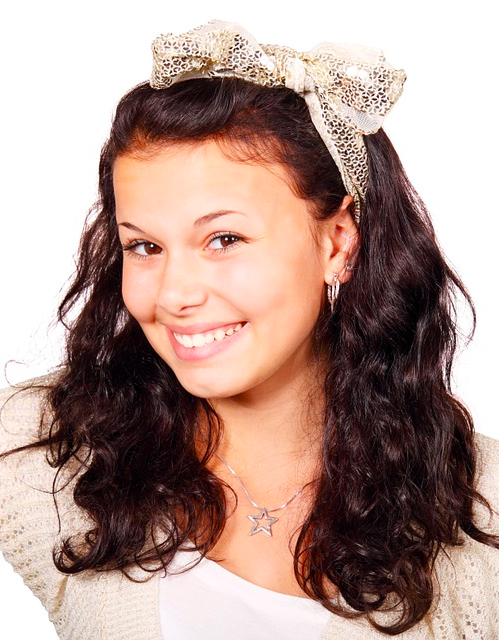
\includegraphics[width=0.21\textwidth]{images/em_white}
\end{figure}
\textbf{Emily White, 18}\\
\textbf{Description}: Emily has just started at the University of Southampton as a first year student studying History. She has just finished college and does not know many people at the university. All the information presented to her in the first few weeks of university has been very difficult to remember. She comes from a small town and is finding Southampton very big and confusing. She has been struggling with finding the different buildings at the uni and local amenities.\\ 

\textbf{Goals}: Emily needs an application specifically designed for students of the university of Southampton so that she can have access to both her university life and her social life. She would prefer an application where she would ask specific questions and receive customised answers instead of her having to go on Google and having to research specific information.\\

\begin{figure}[H]
	\centering
    
\includegraphics[width=0.22\textwidth]{images/ra_patel}
\end{figure}
\textbf{Rajesh Patel, 21}\\
\textbf{Description}: Rajesh is a third year student at the University of Southampton doing Electrical Engineering. He is a fan of trance music and enjoys going out clubbing. He has been a smoker for a few years and enjoys going to the pub for a drink with his friends. In addition, Rajesh is very passionate about his course and enjoys his lectures.\\ 

\textbf{Goals}: Rajesh would need an application that would tell him where the closest pub is when he would want to grab a drink with his friends. Also, he would need an application to tell him where the closest shop that sells cigarettes is. He would prefer to use an application that he is familiar with to get this information as he does not like learning new apps.\\

\begin{figure}[H]
	\centering
    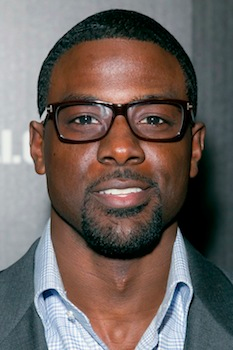
\includegraphics[width=0.2\textwidth]{images/ol_nnachi}
\end{figure}
\textbf{Oluwole Nnachi, 27}\\
\textbf{Description}: Oluwole is an international student at the University of Southampton doing a Masters in Law. He has just moved from Nigeria to the UK and does not know Southampton at all. He is not a very good cook and prefers to eat out in restaurants. He also does not know his way around the university as it is a very big campus which he is not used to in his previous university. He lives very close to the university.\\ 

\textbf{Goals}: Oluwole would like to use an application that showed him where he would be able to have his lunch while he is at the university. Also, as he does not know his way around the university much, it would be very useful if he could find out where every building is and where the nearest amenities are. 

\end{document}